\section{What is Entanglement and what is it good for? \textbf{N}}
	 \begin{figure}[tbp]
	 	\begin{center}
	 		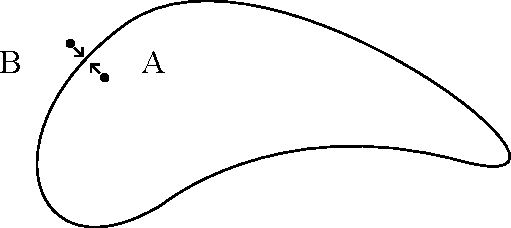
\includegraphics[scale=1]{entangledcorr}
	 		\caption{The boundary between these two regions is called the \textit{entangling surface}.}
	 	\end{center}
	 \end{figure}
	In relativistic QFT, the ground state has correlations between field operators at spatially separated points. Here we can use \textit{entanglement} as an explanation.
	
	But at first, let's start from the beginning:
	\\
	We have $\rho$ which is called \textit{density matrix} and is a quantum state on Hilbert space $\Hil$. Quantum states are illustrated in operators, here: $\rho$ is a non-negative hermitian one of trace 1. If it can be written in the form\footnote{Here $|\psi\rangle$ is some element of $\Hil$ with norm 1.}
		\begin{equation}
			\rho=|\psi\rangle \langle\psi|,
		\end{equation}
	 the quantum state is called \textit{pure}. If a state is not pure, it is \textit{mixed}.
	 
	 While doing an experiment, we will a measure a outcome $i$, which is always related to a projection operator $\Pi_i$ with a probalbility of measuring $i$, that looks like: 
		 \begin{equation}
	 		P(i)=\mathrm{tr}(\rho\Pi_i).
	 	\end{equation}
	 
	 For to find out, whether a given state $\rho$ is pure or mixed, we define a function $S$ for convenience:
		\begin{equation}
			S(\rho)\equiv -\mathrm{tr}(\rho \log \rho)
		\end{equation}	 	
	And $S(\rho)$ is called the \textit{Von Neumann Entropy} or \textit{information entropy}. 
	Its proberties are:
	\begin{itemize}
		\item[•] for any unitary operator $U$: $S(U^\dagger \rho U)=S(\rho)$
		\item[•] $S(\rho)\geq 0$, with equality if and only if $\rho$ is pure. 
		\item[•] for $d$ is the dimension of $\Hil$: $S(\rho)\leq \log d$, with equality if and only if $\rho$ is maximally mixed.
		\item[•] The entropy of the average over a set of states is at least equal to the average of all their individual entropies. This is also called \textit{concavity} and is definde as:
		\begin{equation}
			S \left(\sum_i \lambda_i \rho_i \right) \geq \sum_i \lambda_i S(\rho_i),
		\end{equation}
	while $\lambda_i$ is any set of non-negative numbers with $\sum_i \lambda_i =1$.
	\end{itemize}
	Now, let's have a look at an entangled state written in the two-qubit state:
		\begin{equation}
			|\Psi\rangle = \frac{1}{\sqrt{2}} \left(|00\rangle + |11\rangle \right)
		\end{equation}
	Here, the full state is pure, but the reduced state on either qubit ($|00\rangle$ or $|11\rangle$) is mixed. 
%	Bipartite systems are the ones whose Hilbert space can be written as a tensor product\footnote{Watch out! The tensor product $\otimes$ is not the direct sum $\oplus$.}:
%	 	\begin{equation}
%	 		\Hil=\Hil_A \otimes \Hil_B
%	 	\end{equation}
%	 In quantum mechanics they describe the composition of two independent physical systems and can be \textit{entangled}, which means, that the reduced density matrices $\rho_A$ and $\rho_B$ can be mixed even if the joint state $\rho_{AB}$ is pure.
%	 

\FloatBarrier